\section{Planning Phase}

	This section describes the time leading up to sprint 1, before implementations had started. This phase involved getting to know each other, the customer and the task, as well as making important decisions regarding technologies and development process.

\subsection{Getting to Know Each Other and the Customer}

	The first meeting with the customer took place at the kickoff of the project. 
	The customer introduced the group to their company and their work, but the focus 
	of the meeting was about different ideas for a good concept for the game.
	It was agreed that the group would come up with a game concept and a requirement 
	specification.

\subsection{Project Assignment}
	
	The description of the problem as stated by Helgelandskraft, 
	and found in the course compendium is given below: 
		\paragraph{Power Control Game}
		{\it The idea is to make a casual game for mobile devices focused around controlling 
		power production from hydro plants trough a power grid to large industry customers and 
		regular consumers, or some other casual game involving power grids, hydro plants 
		and/or other themes around hydro power. 
		 
		The application should also provide the user with power preservation tips, like a 
		tip on loading screens or the splash screen when opening the game. Tips like: 
		 
		“19-21 degrees celsius is a good inside temperature. For each degree you lower the temperature 
		you’ll save 5 procent of the energy used for heating up your living space. 
		You can lower the temperature even more in rooms you normally don’t use.” 
		 
		The application should be developed for iOS and Android. We’ll provide the 
		students with the required equipment needed for iOS-development if they don’t 
		have it, and an android phone if they need it. 
		 
		The application should be designed for the tips and the language to easily be changed.}

	Helgelandskraft wanted a game running on Android and iOS, with the main theme "Power".
	In the project description they introduced some key points, but they did not have a
	concrete idea of what they really wanted. The scoping of the project and the developing
	of the game concept was part of the next step.

\subsection{Define the Project Scope}


\subsection{Preliminary studies and Project Planning}
	Soon after the start of the project, the group needed to do research on project methodology, 
	game concepts and technology. This was an important part of the planning seeing as this type of 
	project was new to the group members. The outcome of this research and planning can be found 
	in the 'Project Directive' and 'Preliminary studies'.

	\begin{figure}[H]
		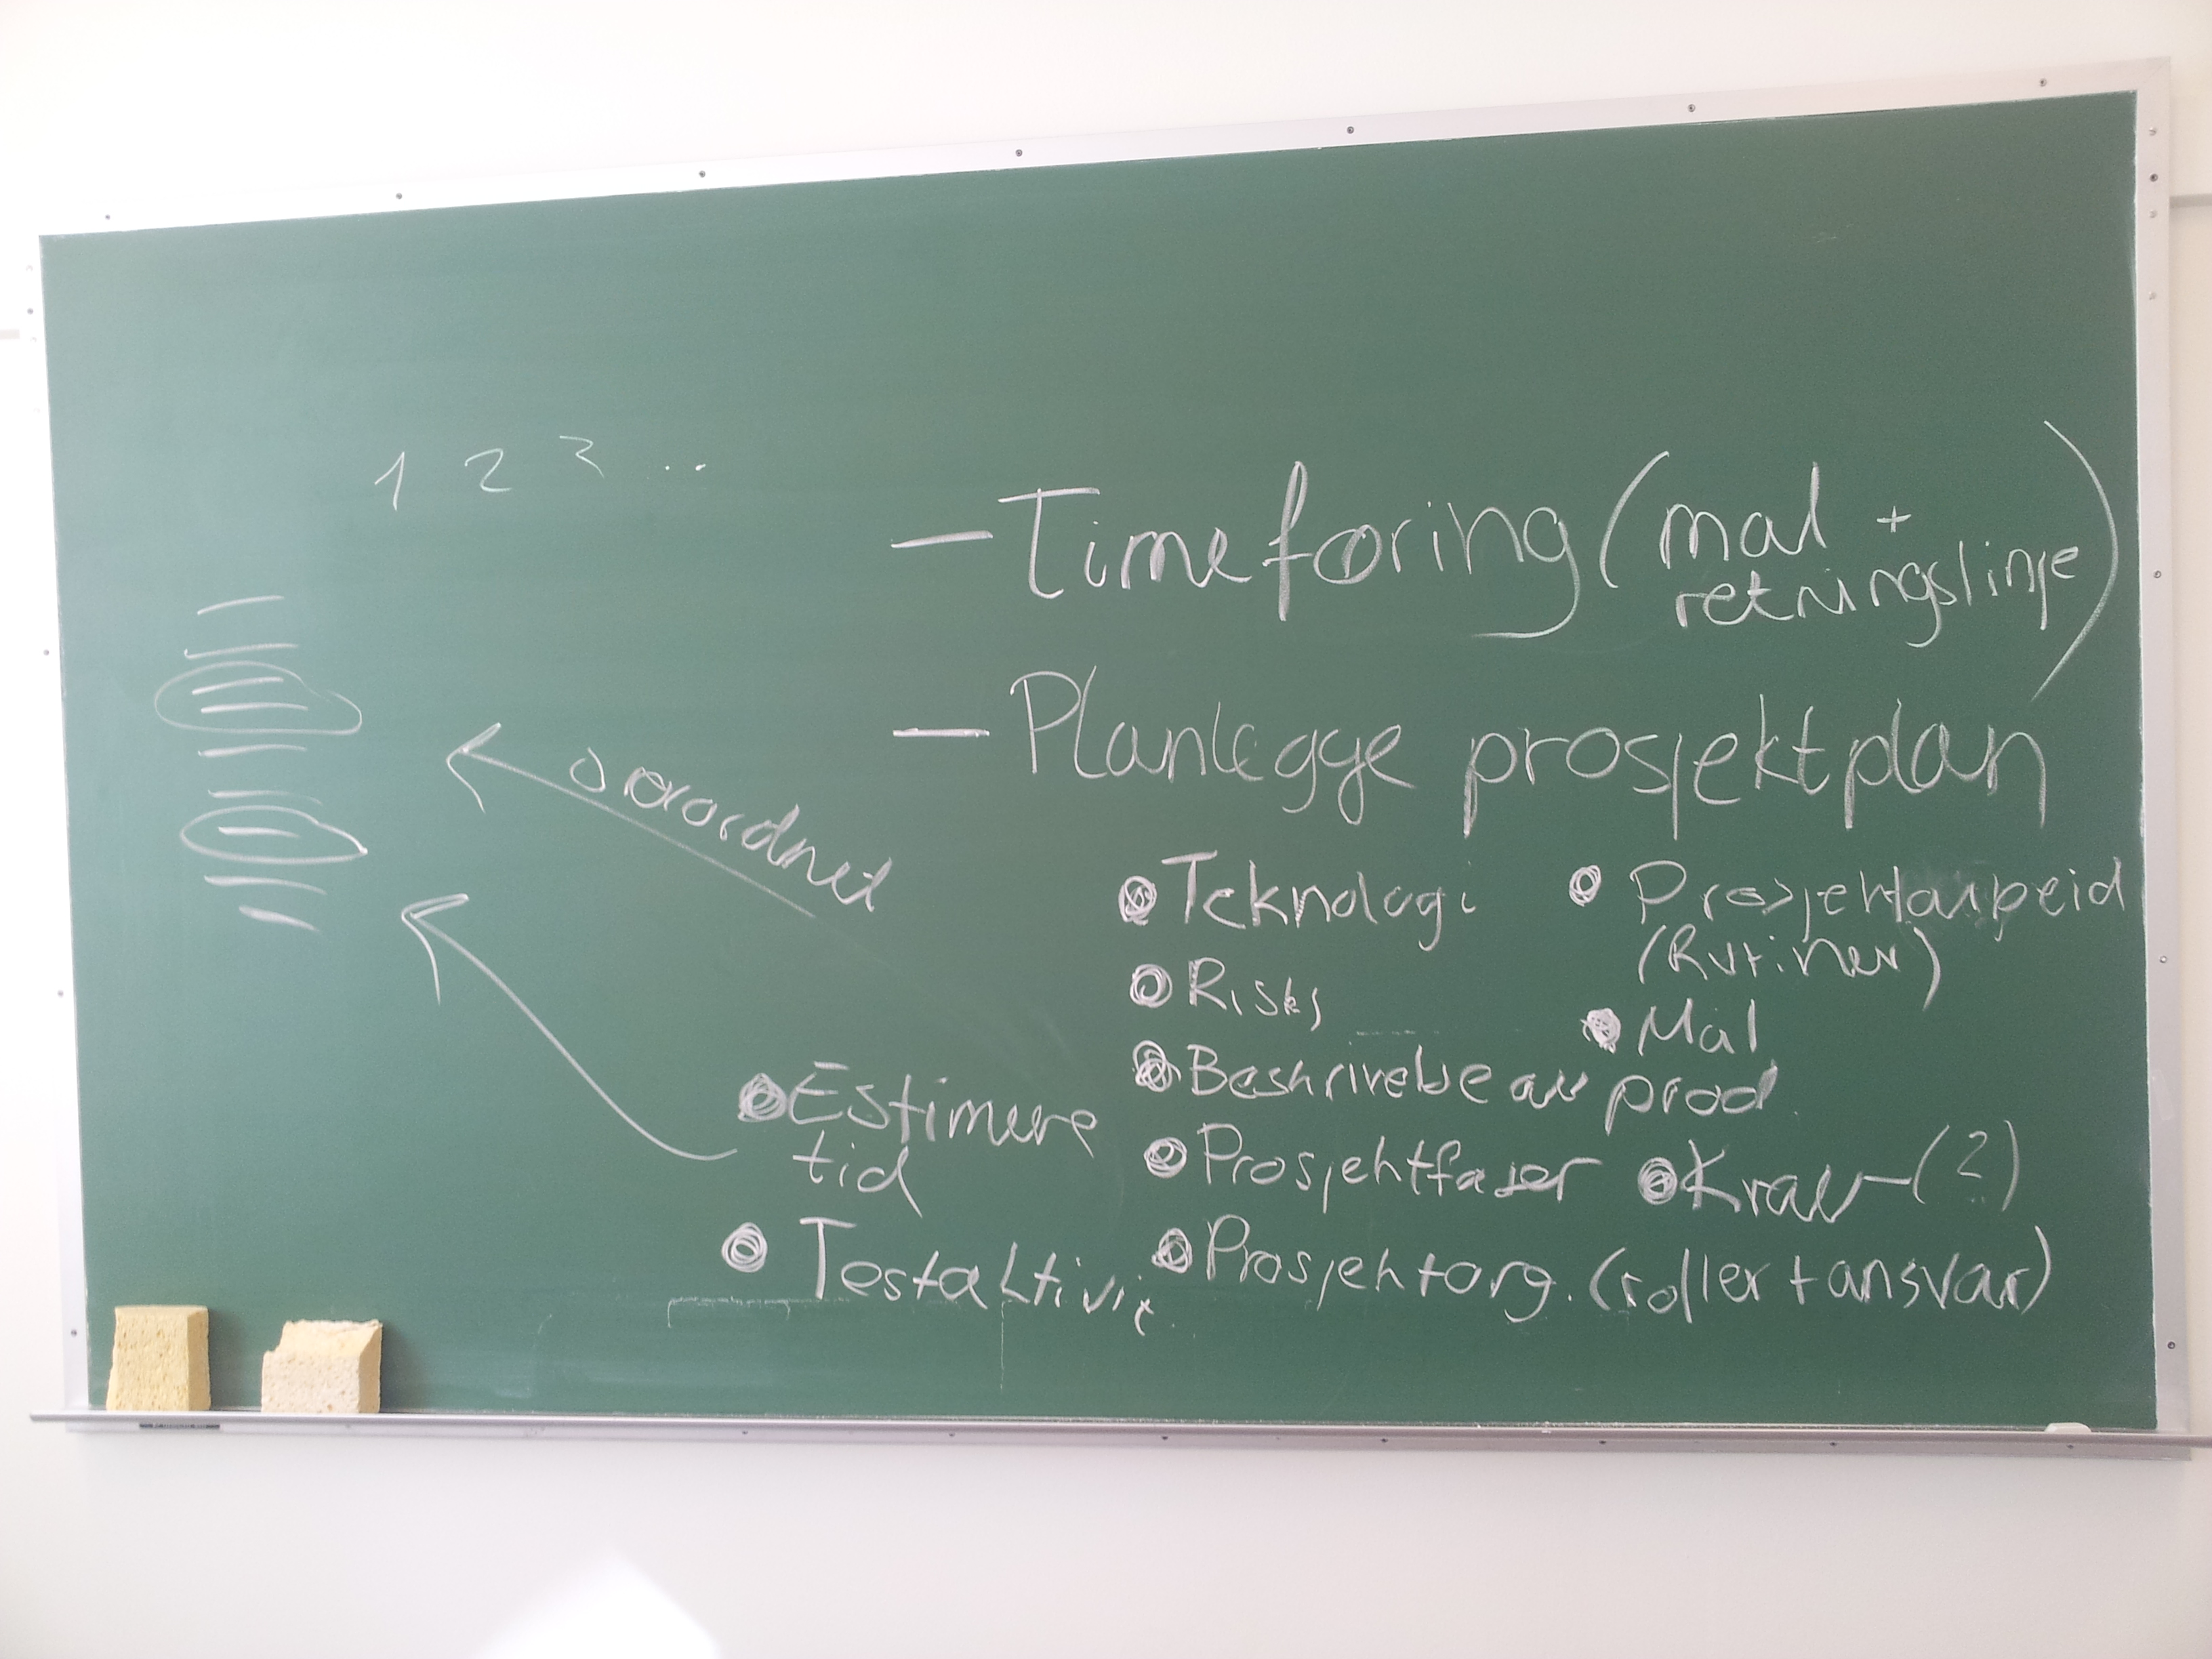
\includegraphics[scale=0.10]{pictures/projectPlanning.jpg}
		\caption{Group planning}
	\end{figure}

\subsection{Game Concept Development}
	
	When trying to come up with a concept for the game the group members sat down in a "green zone". 
	With the green zone concept each team member sat alone for 10 minutes and tried to come up with 
	ideas for a concept. After the 10 minutes all the members presented their ideas to the rest of 
	the team members. After presenting all the concepts, the group took a closer look at the best ideas. 

	The first concept was a "shortest-path-problem" game where the player should
	connect a number of nodes with lines without crossing other lines. The goal 
	was to draw the shortest path between the nodes. When the group presented this
	to the customer, they liked the idea, but they wanted a more "real life" game.

	The next concept was a "sim city" like concept, and was the game concept that
	was chosen do implement. 

	An in depth description of the final concept can be found in the "Game Concept"
	section, and a more detailed description of the coming up with a game concept can 
	be found in "Game Concept Development" under the "Preliminary Studies". 

	\begin{figure}[H]
	\centering
		\subfigure{
			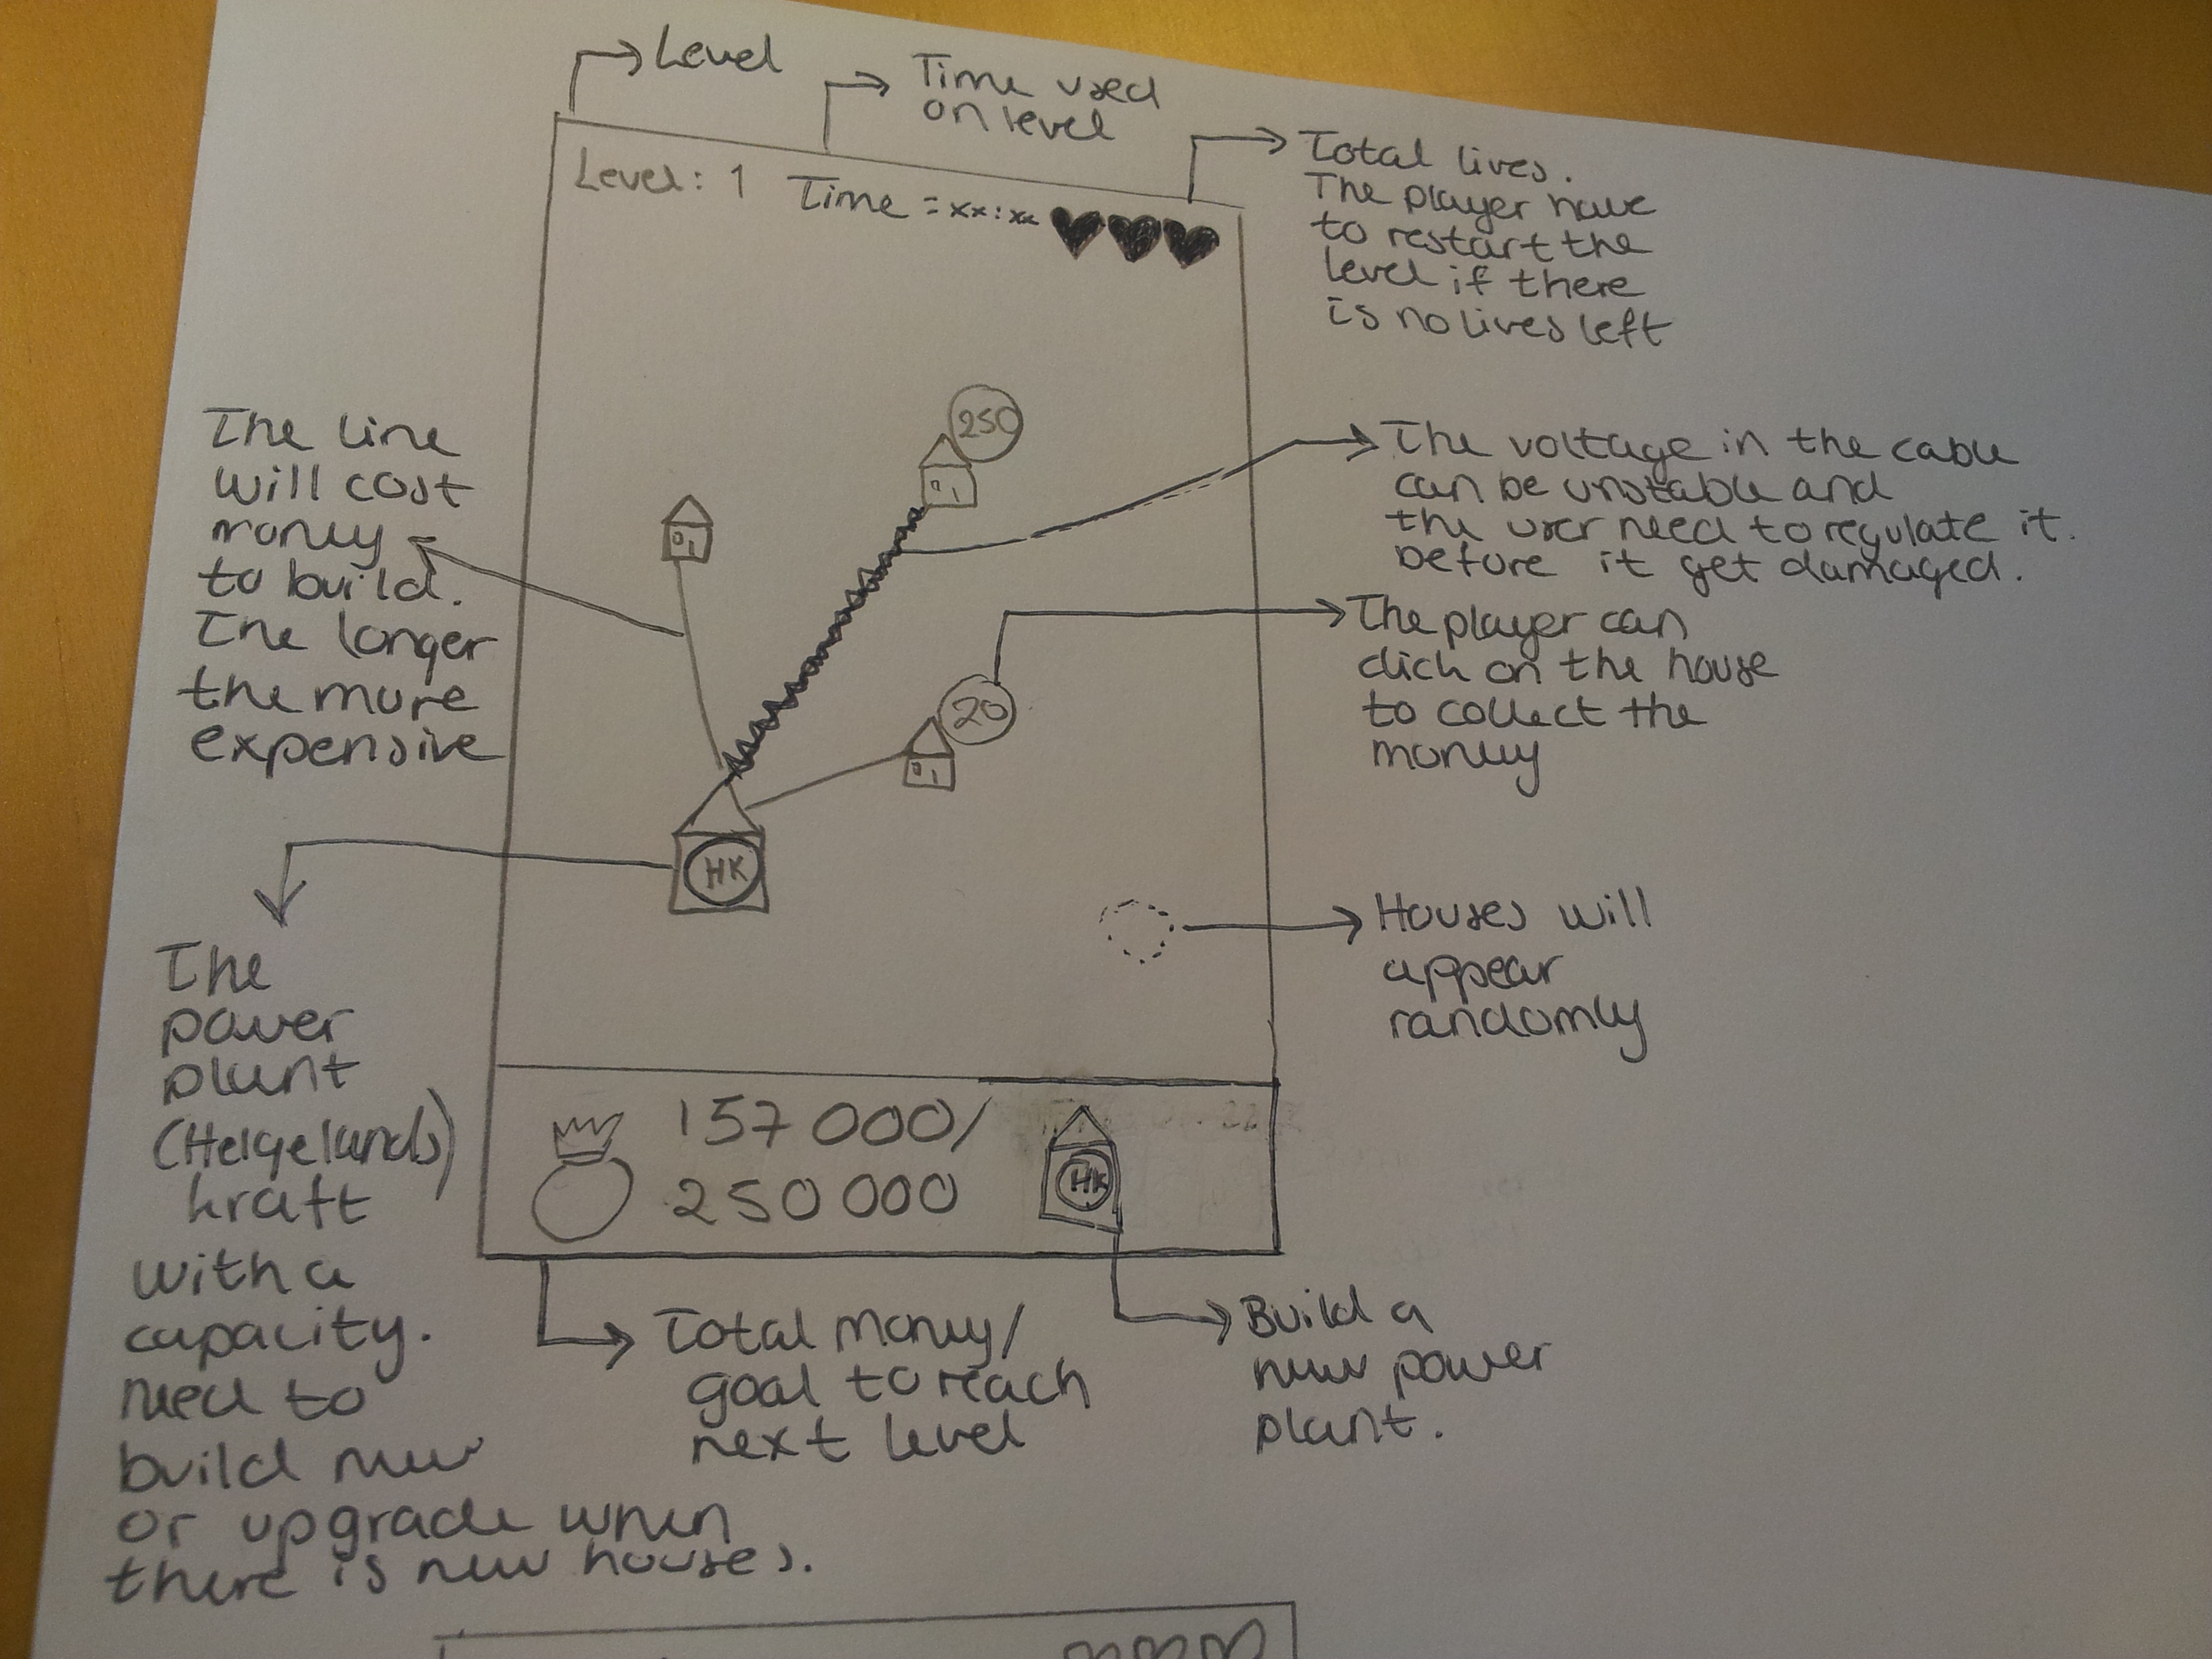
\includegraphics[scale=0.05]{pictures/gameConcept1}
		}
		\subfigure{
			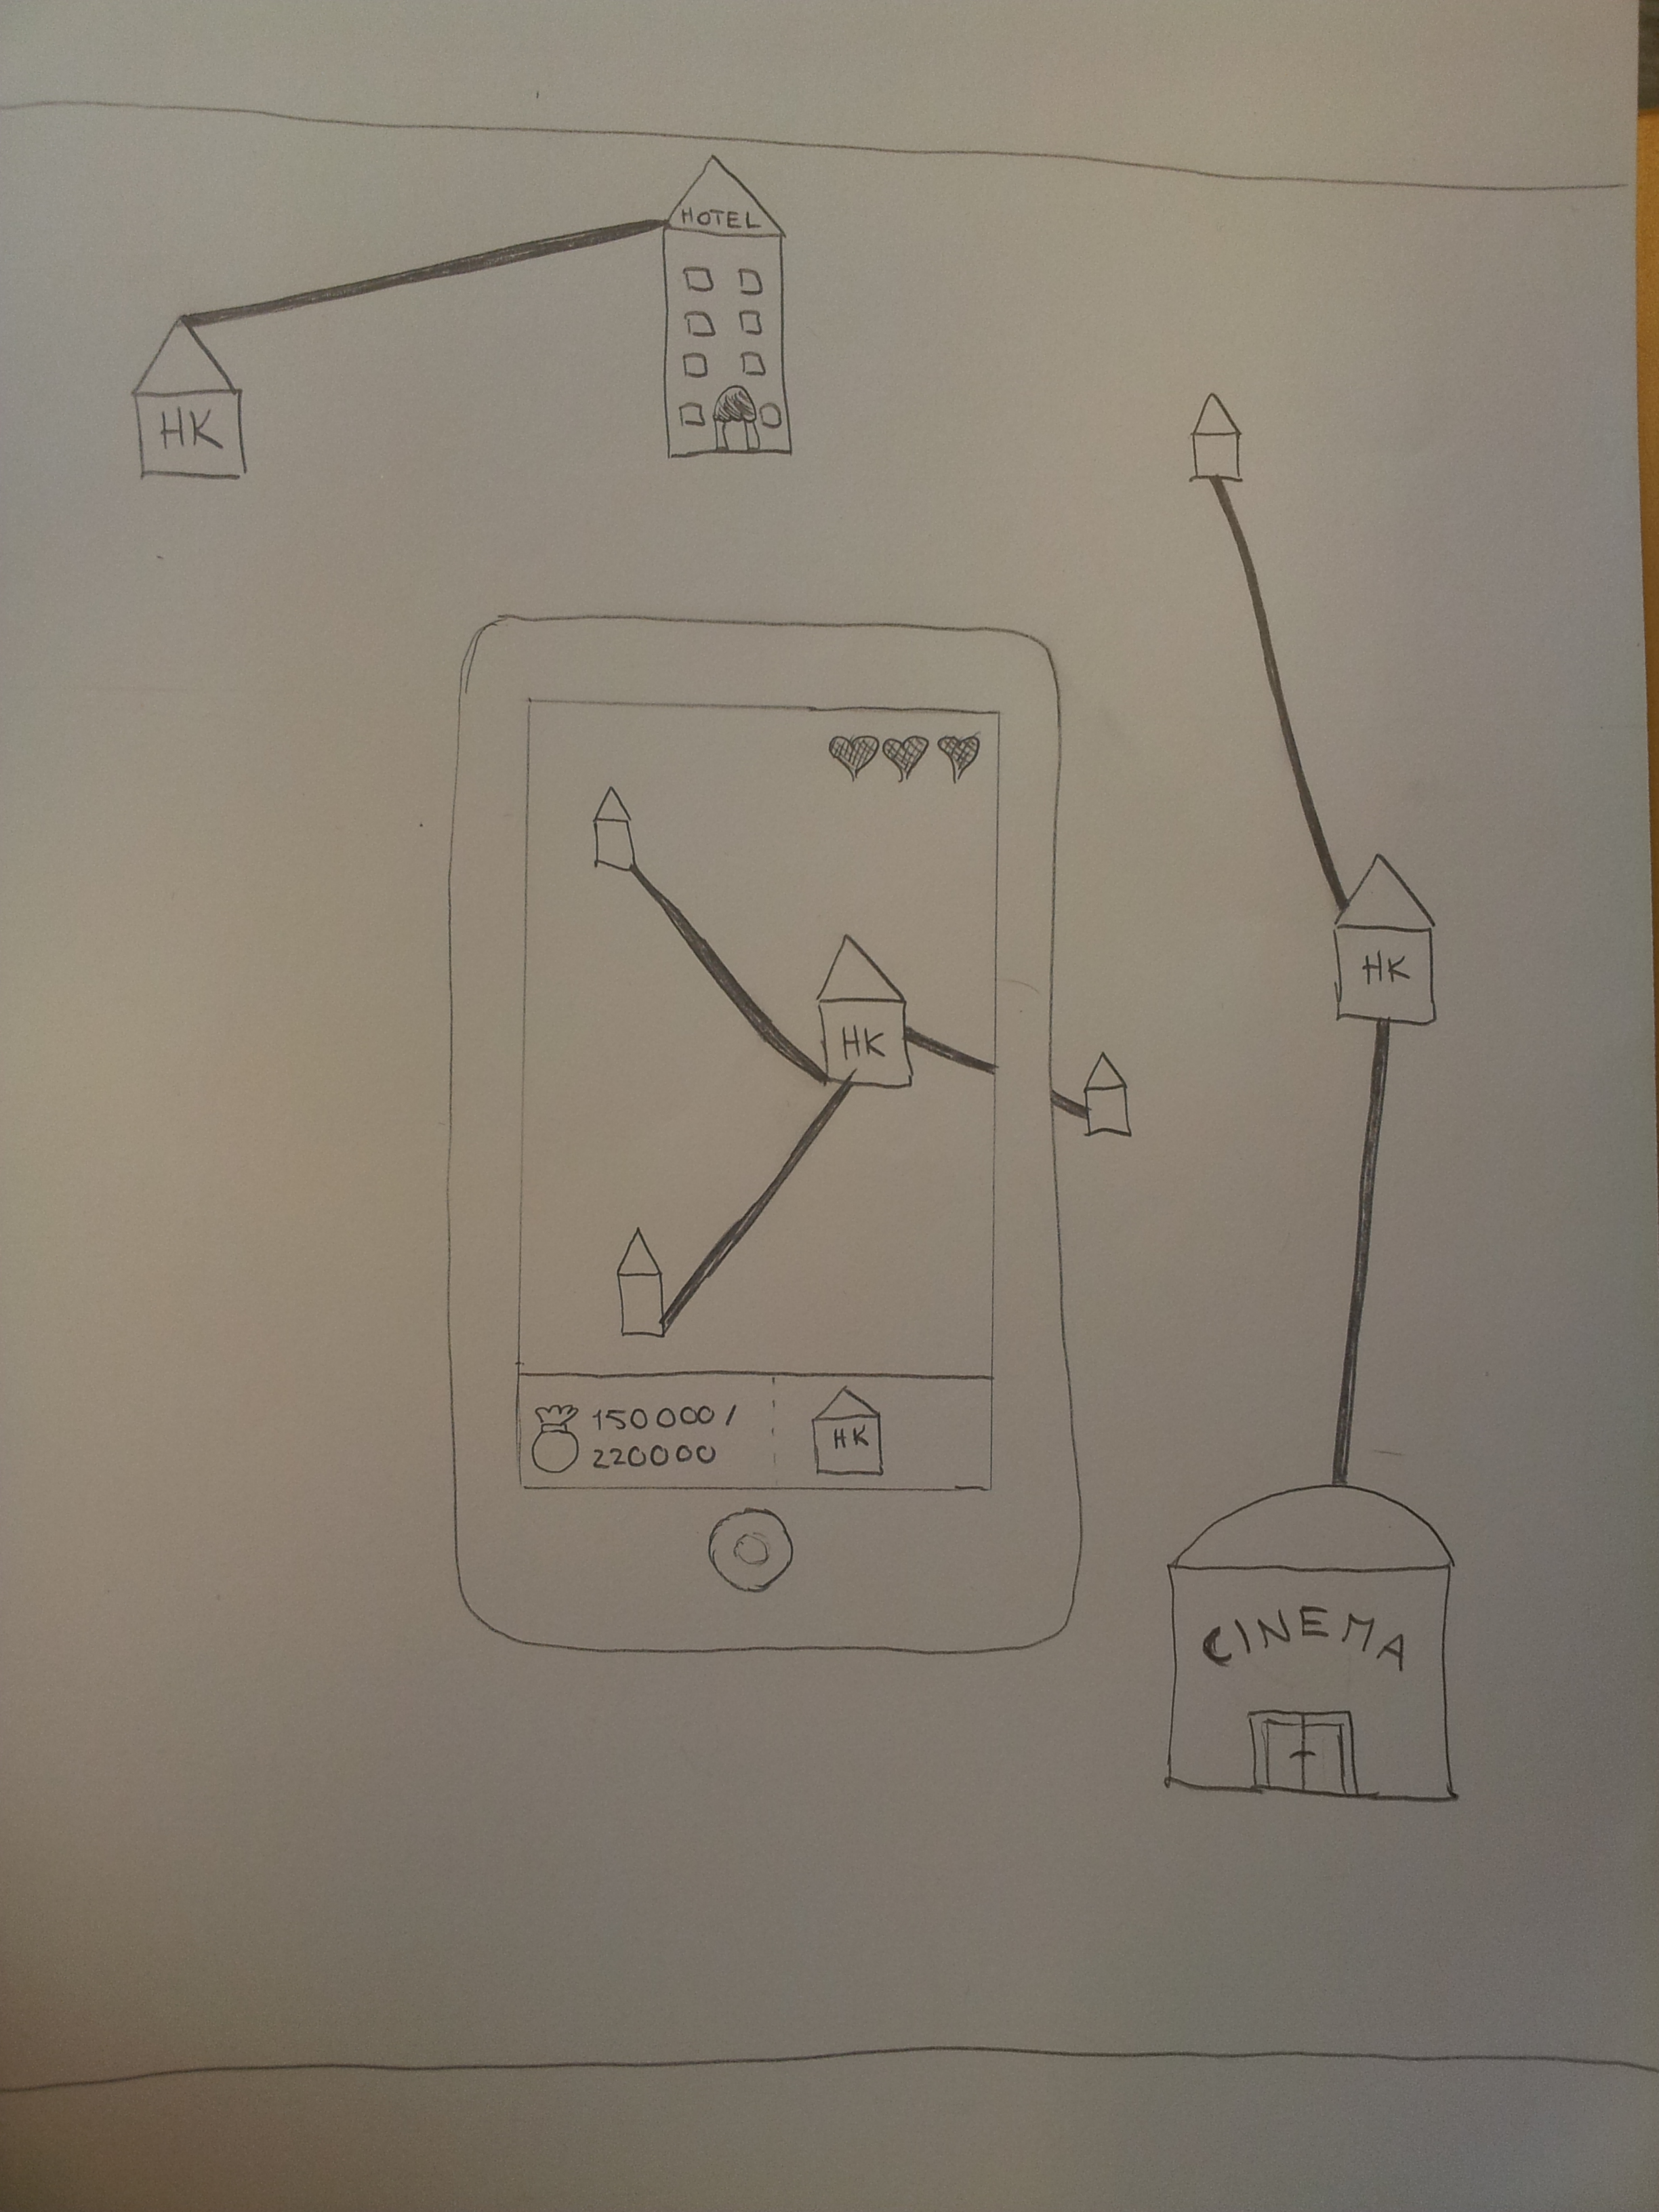
\includegraphics[scale=0.05]{pictures/gameConcept2}
		}
		\caption{Game concept development}
	\end{figure}

\subsection{Specification of the Requirements}
	After the game concept had been approved by the customer, the next step was to 
	get a clear list of all requirements for the game. 

	The requirement specification consists of functional and non-functional requirements to
	fulfill in the project. All the functional requirements have a priority as well as a 
	complexity factor assigned. When the requirement specification was made quite 
	ambitious, so each requirement was registered with a priority from critical to low. 
	The customer was made aware that it might not be time to implement all of the requirements, 
	but that they would be implemented in the order from critical to low. 

	The requirement specification was read and signed by the customer in order give the customer 
	an impression of what they could expect in the final delivery.

\subsection{Duration and workload}
	In the start of this phase, the scrum master made a template for hour registration so that all the group members
	could register all work done in the project. In each phase activities were defined and each
	person registered hours spent on specific activities. Here is the template 
	that were made:

	\begin{figure}[H]
		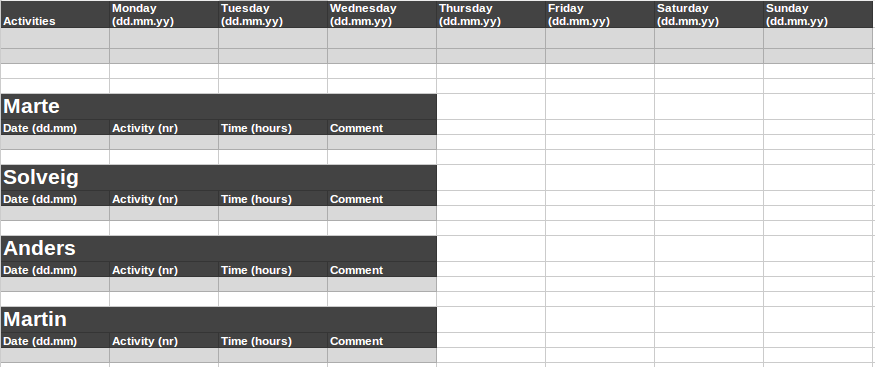
\includegraphics[width=\textwidth]{pictures/timetable.png}
		\caption{Timetable}
	\end{figure}

	The main work was spent on the planning activity. Implementation had not started, and 
	the development activity was spent on preliminary studies for the implementation.

		{\bf Duration:} 09.09 - 29.09 (3 weeks)\\
		{\bf Workload:} This is the list with hours spent (by the whole group) on the project in this phase.
			\begin{itemize}
				\item {\bf Planning:} 99.5 hours
				\item {\bf Development (pre-study):} 25.5 hours
				\item {\bf Design:} 0 hours
				\item {\bf Documentation (report):} 24.5 hours
				\item {\bf Testing:} 0 hour
			\end{itemize}
		{\bf Total workload: } 149.5 hours \\
	The group's goal was to work at least 20 hours pr/person every week. We did not manage this in this phase, but had a average of 18,7 hours each week pr person (149.5 hours/4 persons/2 weeks = 18.7 hours). 
	The main reason for not working as much as wanted was because many of the team member had voluntary
	work at organizations such as UKA, Samfundet and Abakus. This risk is mentioned in the risk assessment. The group 
	hope to be able to work more the next sprints in order to finish the project and the report at the estimated
	time. 

\subsection{Group Dynamics}
	When entering the project, none of the group members knew each other, and we spent a lot
	of time getting to know each other better.

	The group work is initiated by the scrum master and the response in discussions are quite low.
	It can be a problem for the project if the low response in discussions 
	continue in following sprints. This is still at a early point in the project and the group might need
	some more time to get the chance to find a good way to work with each other. 
	We have registered the problem and had a dialog with the supervisor about it. 

\subsection{Phase Results}
	In the end of this sprint
